% Options for packages loaded elsewhere
\PassOptionsToPackage{unicode}{hyperref}
\PassOptionsToPackage{hyphens}{url}
%
\documentclass[
  ignorenonframetext,
]{beamer}
\usepackage{pgfpages}
\setbeamertemplate{caption}[numbered]
\setbeamertemplate{caption label separator}{: }
\setbeamercolor{caption name}{fg=normal text.fg}
\beamertemplatenavigationsymbolsempty
% Prevent slide breaks in the middle of a paragraph
\widowpenalties 1 10000
\raggedbottom
\setbeamertemplate{part page}{
  \centering
  \begin{beamercolorbox}[sep=16pt,center]{part title}
    \usebeamerfont{part title}\insertpart\par
  \end{beamercolorbox}
}
\setbeamertemplate{section page}{
  \centering
  \begin{beamercolorbox}[sep=12pt,center]{part title}
    \usebeamerfont{section title}\insertsection\par
  \end{beamercolorbox}
}
\setbeamertemplate{subsection page}{
  \centering
  \begin{beamercolorbox}[sep=8pt,center]{part title}
    \usebeamerfont{subsection title}\insertsubsection\par
  \end{beamercolorbox}
}
\AtBeginPart{
  \frame{\partpage}
}
\AtBeginSection{
  \ifbibliography
  \else
    \frame{\sectionpage}
  \fi
}
\AtBeginSubsection{
  \frame{\subsectionpage}
}
\usepackage{amsmath,amssymb}
\usepackage{iftex}
\ifPDFTeX
  \usepackage[T1]{fontenc}
  \usepackage[utf8]{inputenc}
  \usepackage{textcomp} % provide euro and other symbols
\else % if luatex or xetex
  \usepackage{unicode-math} % this also loads fontspec
  \defaultfontfeatures{Scale=MatchLowercase}
  \defaultfontfeatures[\rmfamily]{Ligatures=TeX,Scale=1}
\fi
\usepackage{lmodern}
\usetheme[]{default}
\usefonttheme{professionalfonts}
\ifPDFTeX\else
  % xetex/luatex font selection
\fi
% Use upquote if available, for straight quotes in verbatim environments
\IfFileExists{upquote.sty}{\usepackage{upquote}}{}
\IfFileExists{microtype.sty}{% use microtype if available
  \usepackage[]{microtype}
  \UseMicrotypeSet[protrusion]{basicmath} % disable protrusion for tt fonts
}{}
\makeatletter
\@ifundefined{KOMAClassName}{% if non-KOMA class
  \IfFileExists{parskip.sty}{%
    \usepackage{parskip}
  }{% else
    \setlength{\parindent}{0pt}
    \setlength{\parskip}{6pt plus 2pt minus 1pt}}
}{% if KOMA class
  \KOMAoptions{parskip=half}}
\makeatother
\usepackage{xcolor}
\newif\ifbibliography
\usepackage{graphicx}
\makeatletter
\def\maxwidth{\ifdim\Gin@nat@width>\linewidth\linewidth\else\Gin@nat@width\fi}
\def\maxheight{\ifdim\Gin@nat@height>\textheight\textheight\else\Gin@nat@height\fi}
\makeatother
% Scale images if necessary, so that they will not overflow the page
% margins by default, and it is still possible to overwrite the defaults
% using explicit options in \includegraphics[width, height, ...]{}
\setkeys{Gin}{width=\maxwidth,height=\maxheight,keepaspectratio}
% Set default figure placement to htbp
\makeatletter
\def\fps@figure{htbp}
\makeatother
\setlength{\emergencystretch}{3em} % prevent overfull lines
\providecommand{\tightlist}{%
  \setlength{\itemsep}{0pt}\setlength{\parskip}{0pt}}
\setcounter{secnumdepth}{-\maxdimen} % remove section numbering
\usepackage{fancyhdr}
\usepackage{lastpage}
\setbeamertemplate{navigation symbols}{}
\setbeamertemplate{footline}[page number]
\pagenumbering{arabic}
% \usepackage[mathbf,mathcal]{euler}

\ifLuaTeX
  \usepackage{selnolig}  % disable illegal ligatures
\fi
\IfFileExists{bookmark.sty}{\usepackage{bookmark}}{\usepackage{hyperref}}
\IfFileExists{xurl.sty}{\usepackage{xurl}}{} % add URL line breaks if available
\urlstyle{same}
\hypersetup{
  hidelinks,
  pdfcreator={LaTeX via pandoc}}

\title{Experimentos de Encuestas - Qualtrics}
\author{Luciana Cantera\\
Diseño e implementación de experimentos en ciencias sociales\\
\emph{Departamento de Economía (UdelaR)}}
\date{}

\begin{document}
\frame{\titlepage}

\begin{frame}{Qualtrics}
\protect\hypertarget{qualtrics}{}
Herramienta versátil y de manejo sencillo que permite elaborar
cuestionarios online, para ser utilizados en estudios de encuesta y
experimentos
\end{frame}

\begin{frame}{Crear cuenta}
\protect\hypertarget{crear-cuenta}{}
\begin{enumerate}
\item
  Ingresar a:
  \url{https://www.qualtrics.com/free-account/?utm_lp=login-banner}
\item
  Crear una cuenta
\end{enumerate}
\end{frame}

\begin{frame}{Importar experimento}
\protect\hypertarget{importar-experimento}{}
\begin{enumerate}
\setcounter{enumi}{2}
\item
  Ingresar al usuario
\item
  Ir a ``Projects''
\item
  Create project
\item
  Seleccionar ``Survey'' - Get start
\item
  Completar ``Name'' y ``Folder''
\item
  Donde dice ``How do you want to start your survey?'' seleccionar
  ``Import a QSF file''
\item
  Chose file: ``Experimentos\_de\_encuesta.qsf''
\item
  Seleccionar ``Create project''
\end{enumerate}
\end{frame}

\begin{frame}{Encuesta - Inicio}
\protect\hypertarget{encuesta---inicio}{}
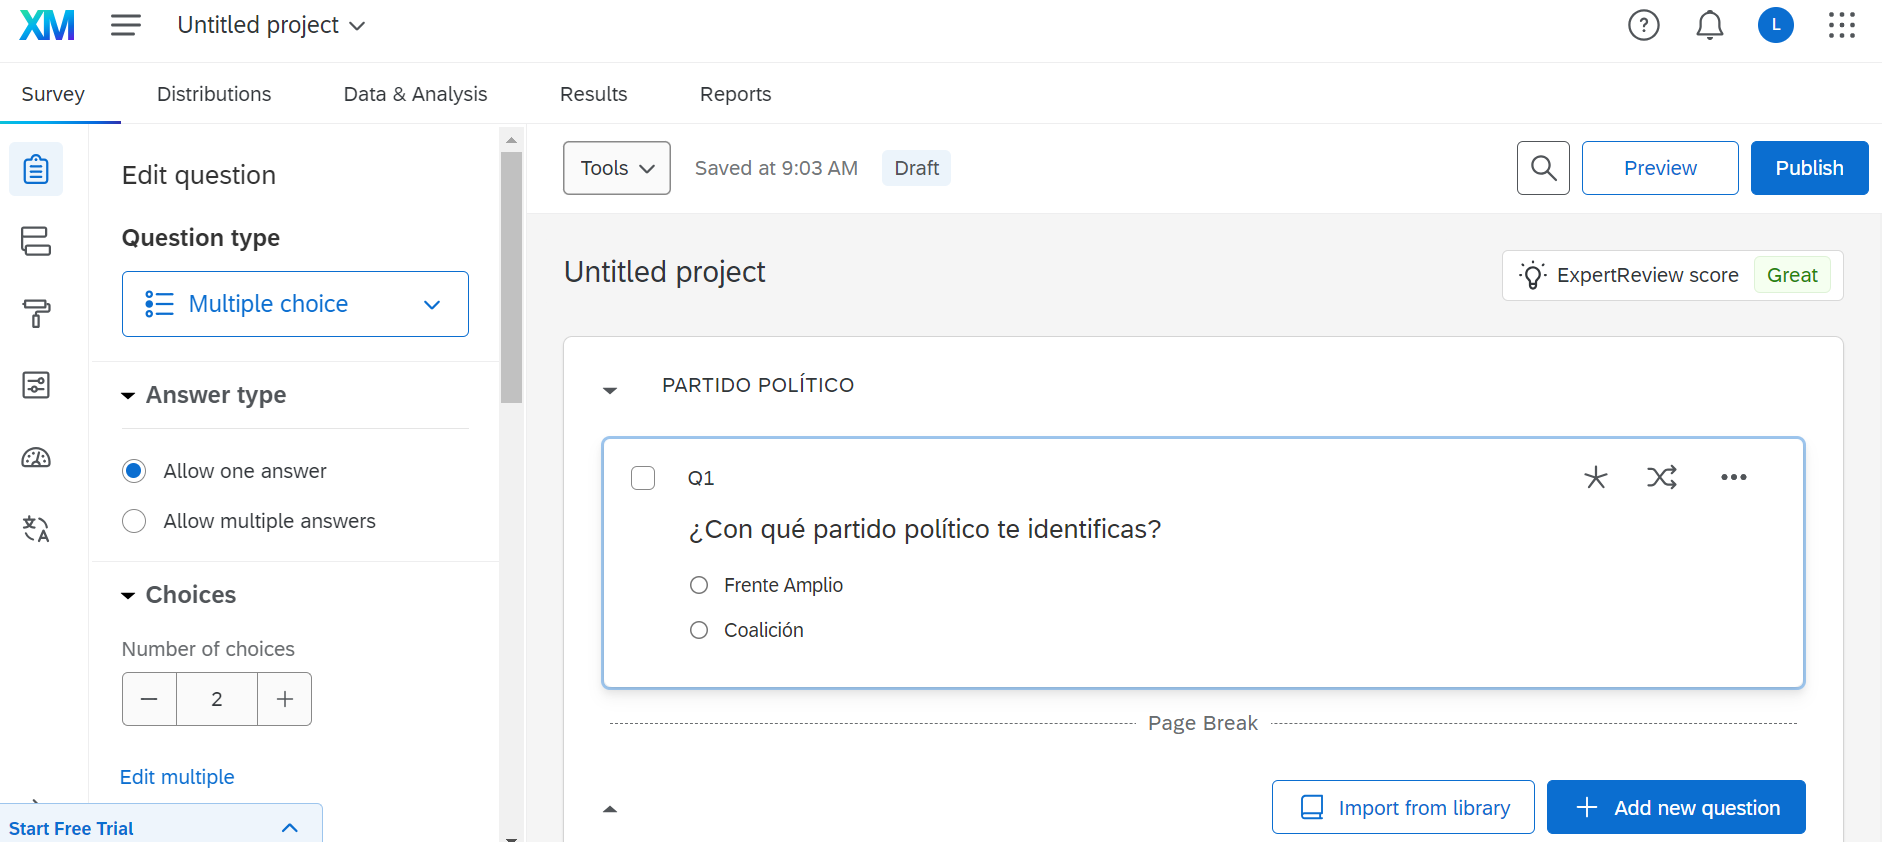
\includegraphics{figs/Qualtrics_survey.png}
\end{frame}

\begin{frame}{Encuesta - Survey Flow}
\protect\hypertarget{encuesta---survey-flow}{}
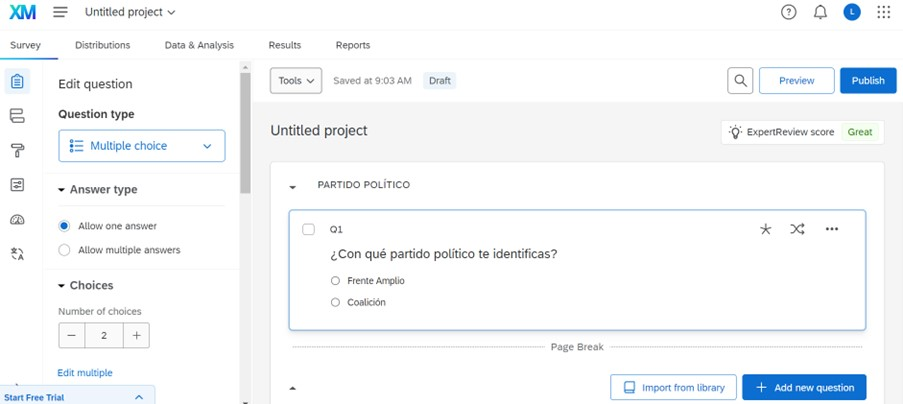
\includegraphics{figs/Qualtrics_survey flow.jpg}
\end{frame}

\begin{frame}{Qualtrics}
\protect\hypertarget{qualtrics-1}{}
\begin{itemize}
\item
  Randomizer:
  \url{https://www.qualtrics.com/support/survey-platform/survey-module/survey-flow/standard-elements/randomizer/}
\item
  Embedded data:
  \url{https://www.qualtrics.com/support/survey-platform/survey-module/survey-flow/standard-elements/embedded-data/}
\item
  Branch logic:
  \url{https://www.qualtrics.com/support/survey-platform/survey-module/survey-flow/standard-elements/branch-logic/}
\item
  Question randomization:
  \url{https://www.qualtrics.com/support/survey-platform/survey-module/block-options/question-randomization/}
\item
  Display logic:
  \url{https://www.qualtrics.com/support/survey-platform/survey-module/question-options/display-logic/}
\end{itemize}
\end{frame}

\begin{frame}{Ejercicio 1 - Diseño del Experimento}
\protect\hypertarget{ejercicio-1---diseuxf1o-del-experimento}{}
\begin{enumerate}
\item
  Realizar un sorteo en el survey flow para dividir a quienes realizan
  la encuesta en dos grupos (T1 y T2). (Randomizer y Embedded Data)
\item
  Asignar un tratamiento a la mitad de los encuestados (Block 1) y el
  otro tratamiento a los restantes (Block 2). (Branch logic)
\item
  Dentro del bloque 1 y bloque 2, indicar que aparezca la pregunta que
  corresponde según lo que respondieron en Q1. (Display logic)
\item
  Aleatorizar el orden en que aparecen las opciones de respuestas en las
  preguntas Q1 y Q10 (Question randomization)
\item
  Manipulation check: Condicionar para que aparezca la opción contraria
  a lo que respondieron en la pregunta 1 (Display Logic)
\end{enumerate}
\end{frame}

\begin{frame}{Ejercicio 2 - Grupo control y/o placebo}
\protect\hypertarget{ejercicio-2---grupo-control-yo-placebo}{}
\begin{enumerate}
\item
  Grupo Control: Incorporar un nuevo grupo en el sorteo que no reciba
  ningun tratamiento
\item
  Placebo:

  \begin{enumerate}
  [a.]
  \tightlist
  \item
    generar una nueva pregunta ``Placebo''
  \item
    incorporar un nuevo grupo en el sorteo y asignar a ese grupo para
    que reciba el placebo
  \end{enumerate}
\end{enumerate}
\end{frame}

\end{document}
